\documentclass[twoside]{book}

% Packages required by doxygen
\usepackage{fixltx2e}
\usepackage{calc}
\usepackage{doxygen}
\usepackage[export]{adjustbox} % also loads graphicx
\usepackage{graphicx}
\usepackage[utf8]{inputenc}
\usepackage{makeidx}
\usepackage{multicol}
\usepackage{multirow}
\PassOptionsToPackage{warn}{textcomp}
\usepackage{textcomp}
\usepackage[nointegrals]{wasysym}
\usepackage[table]{xcolor}

% Font selection
\usepackage[T1]{fontenc}
\usepackage[scaled=.90]{helvet}
\usepackage{courier}
\usepackage{amssymb}
\usepackage{sectsty}
\renewcommand{\familydefault}{\sfdefault}
\allsectionsfont{%
  \fontseries{bc}\selectfont%
  \color{darkgray}%
}
\renewcommand{\DoxyLabelFont}{%
  \fontseries{bc}\selectfont%
  \color{darkgray}%
}
\newcommand{\+}{\discretionary{\mbox{\scriptsize$\hookleftarrow$}}{}{}}

% Page & text layout
\usepackage{geometry}
\geometry{%
  a4paper,%
  top=2.5cm,%
  bottom=2.5cm,%
  left=2.5cm,%
  right=2.5cm%
}
\tolerance=750
\hfuzz=15pt
\hbadness=750
\setlength{\emergencystretch}{15pt}
\setlength{\parindent}{0cm}
\setlength{\parskip}{3ex plus 2ex minus 2ex}
\makeatletter
\renewcommand{\paragraph}{%
  \@startsection{paragraph}{4}{0ex}{-1.0ex}{1.0ex}{%
    \normalfont\normalsize\bfseries\SS@parafont%
  }%
}
\renewcommand{\subparagraph}{%
  \@startsection{subparagraph}{5}{0ex}{-1.0ex}{1.0ex}{%
    \normalfont\normalsize\bfseries\SS@subparafont%
  }%
}
\makeatother

% Headers & footers
\usepackage{fancyhdr}
\pagestyle{fancyplain}
\fancyhead[LE]{\fancyplain{}{\bfseries\thepage}}
\fancyhead[CE]{\fancyplain{}{}}
\fancyhead[RE]{\fancyplain{}{\bfseries\leftmark}}
\fancyhead[LO]{\fancyplain{}{\bfseries\rightmark}}
\fancyhead[CO]{\fancyplain{}{}}
\fancyhead[RO]{\fancyplain{}{\bfseries\thepage}}
\fancyfoot[LE]{\fancyplain{}{}}
\fancyfoot[CE]{\fancyplain{}{}}
\fancyfoot[RE]{\fancyplain{}{\bfseries\scriptsize Generated by Doxygen }}
\fancyfoot[LO]{\fancyplain{}{\bfseries\scriptsize Generated by Doxygen }}
\fancyfoot[CO]{\fancyplain{}{}}
\fancyfoot[RO]{\fancyplain{}{}}
\renewcommand{\footrulewidth}{0.4pt}
\renewcommand{\chaptermark}[1]{%
  \markboth{#1}{}%
}
\renewcommand{\sectionmark}[1]{%
  \markright{\thesection\ #1}%
}

% Indices & bibliography
\usepackage{natbib}
\usepackage[titles]{tocloft}
\setcounter{tocdepth}{3}
\setcounter{secnumdepth}{5}
\makeindex

% Hyperlinks (required, but should be loaded last)
\usepackage{ifpdf}
\ifpdf
  \usepackage[pdftex,pagebackref=true]{hyperref}
\else
  \usepackage[ps2pdf,pagebackref=true]{hyperref}
\fi
\hypersetup{%
  colorlinks=true,%
  linkcolor=blue,%
  citecolor=blue,%
  unicode%
}

% Custom commands
\newcommand{\clearemptydoublepage}{%
  \newpage{\pagestyle{empty}\cleardoublepage}%
}

\usepackage{caption}
\captionsetup{labelsep=space,justification=centering,font={bf},singlelinecheck=off,skip=4pt,position=top}

%===== C O N T E N T S =====

\begin{document}

% Titlepage & ToC
\hypersetup{pageanchor=false,
             bookmarksnumbered=true,
             pdfencoding=unicode
            }
\pagenumbering{alph}
\begin{titlepage}
\vspace*{7cm}
\begin{center}%
{\Large My Project }\\
\vspace*{1cm}
{\large Generated by Doxygen 1.8.13}\\
\end{center}
\end{titlepage}
\clearemptydoublepage
\pagenumbering{roman}
\tableofcontents
\clearemptydoublepage
\pagenumbering{arabic}
\hypersetup{pageanchor=true}

%--- Begin generated contents ---
\chapter{Data Structure Index}
\section{Data Structures}
Here are the data structures with brief descriptions\+:\begin{DoxyCompactList}
\item\contentsline{section}{\hyperlink{structentity}{entity} }{\pageref{structentity}}{}
\item\contentsline{section}{\hyperlink{structquiz}{quiz} }{\pageref{structquiz}}{}
\item\contentsline{section}{\hyperlink{structrest}{rest} }{\pageref{structrest}}{}
\end{DoxyCompactList}

\chapter{File Index}
\section{File List}
Here is a list of all files with brief descriptions\+:\begin{DoxyCompactList}
\item\contentsline{section}{\hyperlink{create_8c}{create.\+c} \\*Dans ce fichier deux fichiers binaires fait les appelles }{\pageref{create_8c}}{}
\item\contentsline{section}{\hyperlink{main_8c}{main.\+c} \\*Circuit enigme quiz }{\pageref{main_8c}}{}
\item\contentsline{section}{\hyperlink{quiz_8c}{quiz.\+c} \\*Il y a ici tous les fonctions de l\textquotesingle{}enigme quiz }{\pageref{quiz_8c}}{}
\item\contentsline{section}{\hyperlink{quiz_8h}{quiz.\+h} \\*Il y a ici les structures et la liaison des procedures de l\textquotesingle{}enigme }{\pageref{quiz_8h}}{}
\end{DoxyCompactList}

\chapter{Data Structure Documentation}
\hypertarget{structentity}{}\section{entity Struct Reference}
\label{structentity}\index{entity@{entity}}


{\ttfamily \#include $<$quiz.\+h$>$}

\subsection*{Data Fields}
\begin{DoxyCompactItemize}
\item 
S\+D\+L\+\_\+\+Surface $\ast$ \hyperlink{structentity_a22197c216eb597188b65d419b24abc95}{image}
\item 
S\+D\+L\+\_\+\+Rect \hyperlink{structentity_aa46a7c1001a6a18bca745044952539f7}{pos}
\end{DoxyCompactItemize}


\subsection{Field Documentation}
\mbox{\Hypertarget{structentity_a22197c216eb597188b65d419b24abc95}\label{structentity_a22197c216eb597188b65d419b24abc95}} 
\index{entity@{entity}!image@{image}}
\index{image@{image}!entity@{entity}}
\subsubsection{\texorpdfstring{image}{image}}
{\footnotesize\ttfamily S\+D\+L\+\_\+\+Surface$\ast$ entity\+::image}

\mbox{\Hypertarget{structentity_aa46a7c1001a6a18bca745044952539f7}\label{structentity_aa46a7c1001a6a18bca745044952539f7}} 
\index{entity@{entity}!pos@{pos}}
\index{pos@{pos}!entity@{entity}}
\subsubsection{\texorpdfstring{pos}{pos}}
{\footnotesize\ttfamily S\+D\+L\+\_\+\+Rect entity\+::pos}



The documentation for this struct was generated from the following file\+:\begin{DoxyCompactItemize}
\item 
\hyperlink{quiz_8h}{quiz.\+h}\end{DoxyCompactItemize}

\hypertarget{structquiz}{}\section{quiz Struct Reference}
\label{structquiz}\index{quiz@{quiz}}


{\ttfamily \#include $<$quiz.\+h$>$}



Collaboration diagram for quiz\+:\nopagebreak
\begin{figure}[H]
\begin{center}
\leavevmode
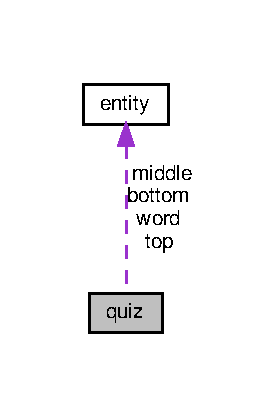
\includegraphics[width=133pt]{structquiz__coll__graph}
\end{center}
\end{figure}
\subsection*{Data Fields}
\begin{DoxyCompactItemize}
\item 
\hyperlink{structentity}{entity} \hyperlink{structquiz_a1b17d6e71182a599abb2a3b721566738}{word}
\item 
\hyperlink{structentity}{entity} \hyperlink{structquiz_ad1183ce4a603358f7f9016913219e775}{top}
\item 
\hyperlink{structentity}{entity} \hyperlink{structquiz_a0528acd950fa1ec3b96679a018272f8c}{middle}
\item 
\hyperlink{structentity}{entity} \hyperlink{structquiz_a9c0a92bdf8150390cff6037818236b66}{bottom}
\end{DoxyCompactItemize}


\subsection{Field Documentation}
\mbox{\Hypertarget{structquiz_a9c0a92bdf8150390cff6037818236b66}\label{structquiz_a9c0a92bdf8150390cff6037818236b66}} 
\index{quiz@{quiz}!bottom@{bottom}}
\index{bottom@{bottom}!quiz@{quiz}}
\subsubsection{\texorpdfstring{bottom}{bottom}}
{\footnotesize\ttfamily \hyperlink{structentity}{entity} quiz\+::bottom}

\mbox{\Hypertarget{structquiz_a0528acd950fa1ec3b96679a018272f8c}\label{structquiz_a0528acd950fa1ec3b96679a018272f8c}} 
\index{quiz@{quiz}!middle@{middle}}
\index{middle@{middle}!quiz@{quiz}}
\subsubsection{\texorpdfstring{middle}{middle}}
{\footnotesize\ttfamily \hyperlink{structentity}{entity} quiz\+::middle}

\mbox{\Hypertarget{structquiz_ad1183ce4a603358f7f9016913219e775}\label{structquiz_ad1183ce4a603358f7f9016913219e775}} 
\index{quiz@{quiz}!top@{top}}
\index{top@{top}!quiz@{quiz}}
\subsubsection{\texorpdfstring{top}{top}}
{\footnotesize\ttfamily \hyperlink{structentity}{entity} quiz\+::top}

\mbox{\Hypertarget{structquiz_a1b17d6e71182a599abb2a3b721566738}\label{structquiz_a1b17d6e71182a599abb2a3b721566738}} 
\index{quiz@{quiz}!word@{word}}
\index{word@{word}!quiz@{quiz}}
\subsubsection{\texorpdfstring{word}{word}}
{\footnotesize\ttfamily \hyperlink{structentity}{entity} quiz\+::word}



The documentation for this struct was generated from the following file\+:\begin{DoxyCompactItemize}
\item 
\hyperlink{quiz_8h}{quiz.\+h}\end{DoxyCompactItemize}

\hypertarget{structrest}{}\section{rest Struct Reference}
\label{structrest}\index{rest@{rest}}


{\ttfamily \#include $<$quiz.\+h$>$}



Collaboration diagram for rest\+:\nopagebreak
\begin{figure}[H]
\begin{center}
\leavevmode
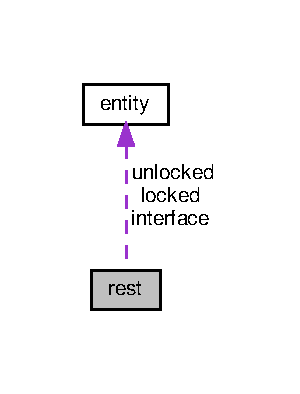
\includegraphics[width=144pt]{structrest__coll__graph}
\end{center}
\end{figure}
\subsection*{Data Fields}
\begin{DoxyCompactItemize}
\item 
\hyperlink{structentity}{entity} \hyperlink{structrest_a063deafa8d3ed41705500b552d9f0e45}{locked}
\item 
\hyperlink{structentity}{entity} \hyperlink{structrest_abdff2c3af489753d37c46a6a2ea318f5}{unlocked}
\item 
\hyperlink{structentity}{entity} \hyperlink{structrest_aa84bc4cd6a7f30715c8dbf1de17b01d0}{interface}
\end{DoxyCompactItemize}


\subsection{Field Documentation}
\mbox{\Hypertarget{structrest_aa84bc4cd6a7f30715c8dbf1de17b01d0}\label{structrest_aa84bc4cd6a7f30715c8dbf1de17b01d0}} 
\index{rest@{rest}!interface@{interface}}
\index{interface@{interface}!rest@{rest}}
\subsubsection{\texorpdfstring{interface}{interface}}
{\footnotesize\ttfamily \hyperlink{structentity}{entity} rest\+::interface}

\mbox{\Hypertarget{structrest_a063deafa8d3ed41705500b552d9f0e45}\label{structrest_a063deafa8d3ed41705500b552d9f0e45}} 
\index{rest@{rest}!locked@{locked}}
\index{locked@{locked}!rest@{rest}}
\subsubsection{\texorpdfstring{locked}{locked}}
{\footnotesize\ttfamily \hyperlink{structentity}{entity} rest\+::locked}

\mbox{\Hypertarget{structrest_abdff2c3af489753d37c46a6a2ea318f5}\label{structrest_abdff2c3af489753d37c46a6a2ea318f5}} 
\index{rest@{rest}!unlocked@{unlocked}}
\index{unlocked@{unlocked}!rest@{rest}}
\subsubsection{\texorpdfstring{unlocked}{unlocked}}
{\footnotesize\ttfamily \hyperlink{structentity}{entity} rest\+::unlocked}



The documentation for this struct was generated from the following file\+:\begin{DoxyCompactItemize}
\item 
\hyperlink{quiz_8h}{quiz.\+h}\end{DoxyCompactItemize}

\chapter{File Documentation}
\hypertarget{create_8c}{}\section{create.\+c File Reference}
\label{create_8c}\index{create.\+c@{create.\+c}}


dans ce fichier deux fichiers binaires fait les appelles.  


{\ttfamily \#include $<$stdio.\+h$>$}\newline
{\ttfamily \#include $<$stdlib.\+h$>$}\newline
{\ttfamily \#include $<$time.\+h$>$}\newline
{\ttfamily \#include \char`\"{}/usr/include/\+S\+D\+L/\+S\+D\+L.\+h\char`\"{}}\newline
{\ttfamily \#include \char`\"{}/usr/include/\+S\+D\+L/\+S\+D\+L\+\_\+image.\+h\char`\"{}}\newline
{\ttfamily \#include \char`\"{}/usr/include/\+S\+D\+L/\+S\+D\+L\+\_\+mixer.\+h\char`\"{}}\newline
{\ttfamily \#include \char`\"{}quiz.\+h\char`\"{}}\newline
Include dependency graph for create.\+c\+:
\nopagebreak
\begin{figure}[H]
\begin{center}
\leavevmode
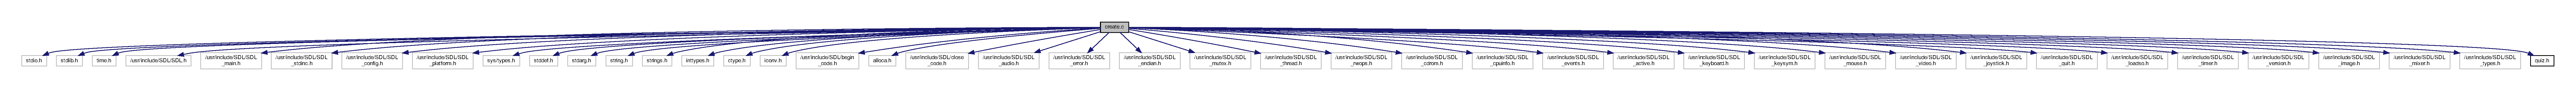
\includegraphics[width=350pt]{create_8c__incl}
\end{center}
\end{figure}
\subsection*{Functions}
\begin{DoxyCompactItemize}
\item 
int \hyperlink{create_8c_a8f387384696c4294f1521ad662b556db}{hover} (S\+D\+L\+\_\+\+Rect pos, int x, int y)
\item 
int \hyperlink{create_8c_ae66f6b31b5ad750f1fe042a706a4e3d4}{main} ()
\end{DoxyCompactItemize}


\subsection{Detailed Description}
dans ce fichier deux fichiers binaires fait les appelles. 



\subsection{Function Documentation}
\mbox{\Hypertarget{create_8c_a8f387384696c4294f1521ad662b556db}\label{create_8c_a8f387384696c4294f1521ad662b556db}} 
\index{create.\+c@{create.\+c}!hover@{hover}}
\index{hover@{hover}!create.\+c@{create.\+c}}
\subsubsection{\texorpdfstring{hover()}{hover()}}
{\footnotesize\ttfamily int hover (\begin{DoxyParamCaption}\item[{S\+D\+L\+\_\+\+Rect}]{pos,  }\item[{int}]{x,  }\item[{int}]{y }\end{DoxyParamCaption})}

\mbox{\Hypertarget{create_8c_ae66f6b31b5ad750f1fe042a706a4e3d4}\label{create_8c_ae66f6b31b5ad750f1fe042a706a4e3d4}} 
\index{create.\+c@{create.\+c}!main@{main}}
\index{main@{main}!create.\+c@{create.\+c}}
\subsubsection{\texorpdfstring{main()}{main()}}
{\footnotesize\ttfamily int main (\begin{DoxyParamCaption}{ }\end{DoxyParamCaption})}


\hypertarget{main_8c}{}\section{main.\+c File Reference}
\label{main_8c}\index{main.\+c@{main.\+c}}


circuit enigme.  


{\ttfamily \#include $<$stdio.\+h$>$}\newline
{\ttfamily \#include $<$stdlib.\+h$>$}\newline
{\ttfamily \#include $<$time.\+h$>$}\newline
{\ttfamily \#include \char`\"{}/usr/include/\+S\+D\+L/\+S\+D\+L.\+h\char`\"{}}\newline
{\ttfamily \#include \char`\"{}/usr/include/\+S\+D\+L/\+S\+D\+L\+\_\+image.\+h\char`\"{}}\newline
{\ttfamily \#include \char`\"{}/usr/include/\+S\+D\+L/\+S\+D\+L\+\_\+mixer.\+h\char`\"{}}\newline
{\ttfamily \#include \char`\"{}/usr/include/\+S\+D\+L/\+S\+D\+L\+\_\+events.\+h\char`\"{}}\newline
{\ttfamily \#include \char`\"{}/usr/include/\+S\+D\+L/\+S\+D\+L\+\_\+mouse.\+h\char`\"{}}\newline
{\ttfamily \#include \char`\"{}circuit.\+h\char`\"{}}\newline
Include dependency graph for main.\+c\+:
\nopagebreak
\begin{figure}[H]
\begin{center}
\leavevmode
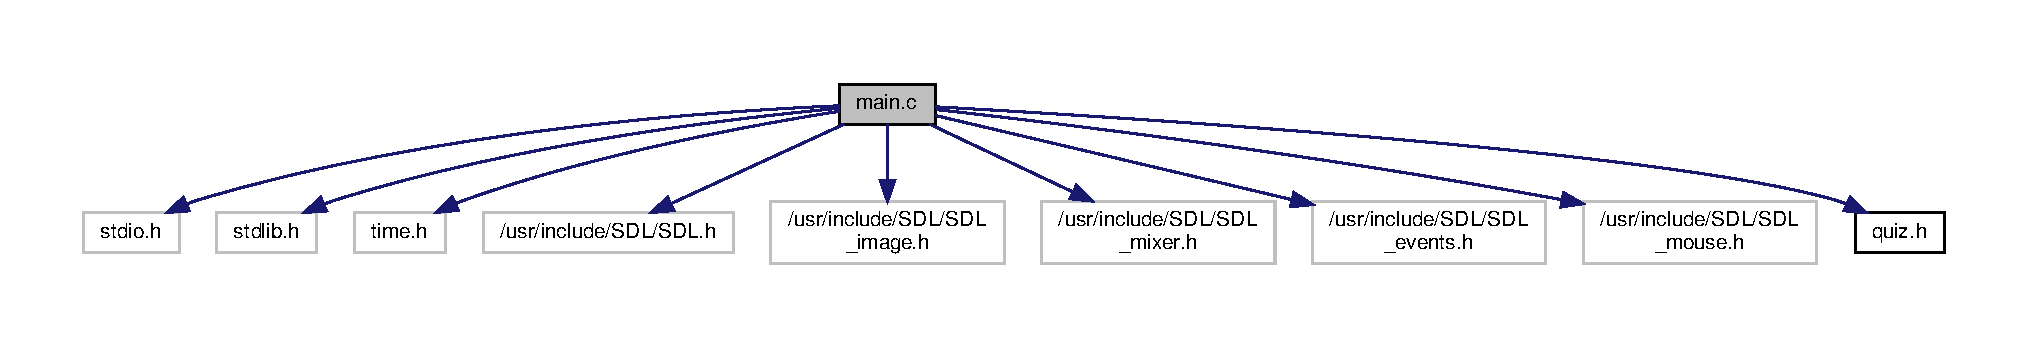
\includegraphics[width=350pt]{main_8c__incl}
\end{center}
\end{figure}
\subsection*{Functions}
\begin{DoxyCompactItemize}
\item 
int \hyperlink{main_8c_ae66f6b31b5ad750f1fe042a706a4e3d4}{main} ()
\end{DoxyCompactItemize}


\subsection{Detailed Description}
circuit enigme. 

\begin{DoxyAuthor}{Author}
Blindspot 
\end{DoxyAuthor}
\begin{DoxyVersion}{Version}
0.\+1 
\end{DoxyVersion}
\begin{DoxyDate}{Date}
M\+AY 06, 2019 
\end{DoxyDate}


\subsection{Function Documentation}
\mbox{\Hypertarget{main_8c_ae66f6b31b5ad750f1fe042a706a4e3d4}\label{main_8c_ae66f6b31b5ad750f1fe042a706a4e3d4}} 
\index{main.\+c@{main.\+c}!main@{main}}
\index{main@{main}!main.\+c@{main.\+c}}
\subsubsection{\texorpdfstring{main()}{main()}}
{\footnotesize\ttfamily int main (\begin{DoxyParamCaption}{ }\end{DoxyParamCaption})}

Here is the call graph for this function\+:\nopagebreak
\begin{figure}[H]
\begin{center}
\leavevmode
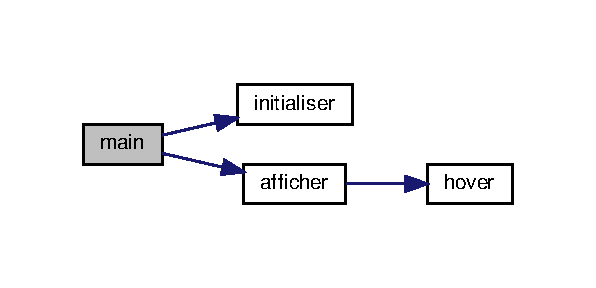
\includegraphics[width=286pt]{main_8c_ae66f6b31b5ad750f1fe042a706a4e3d4_cgraph}
\end{center}
\end{figure}

\hypertarget{quiz_8c}{}\section{quiz.\+c File Reference}
\label{quiz_8c}\index{quiz.\+c@{quiz.\+c}}


il y a ici tous les fonctions de l\textquotesingle{}enigme quiz.  


{\ttfamily \#include $<$stdio.\+h$>$}\newline
{\ttfamily \#include $<$stdlib.\+h$>$}\newline
{\ttfamily \#include $<$time.\+h$>$}\newline
{\ttfamily \#include \char`\"{}/usr/include/\+S\+D\+L/\+S\+D\+L.\+h\char`\"{}}\newline
{\ttfamily \#include \char`\"{}/usr/include/\+S\+D\+L/\+S\+D\+L\+\_\+image.\+h\char`\"{}}\newline
{\ttfamily \#include \char`\"{}/usr/include/\+S\+D\+L/\+S\+D\+L\+\_\+mixer.\+h\char`\"{}}\newline
{\ttfamily \#include \char`\"{}/usr/include/\+S\+D\+L/\+S\+D\+L\+\_\+events.\+h\char`\"{}}\newline
{\ttfamily \#include \char`\"{}/usr/include/\+S\+D\+L/\+S\+D\+L\+\_\+mouse.\+h\char`\"{}}\newline
{\ttfamily \#include \char`\"{}quiz.\+h\char`\"{}}\newline
Include dependency graph for quiz.\+c\+:
\nopagebreak
\begin{figure}[H]
\begin{center}
\leavevmode
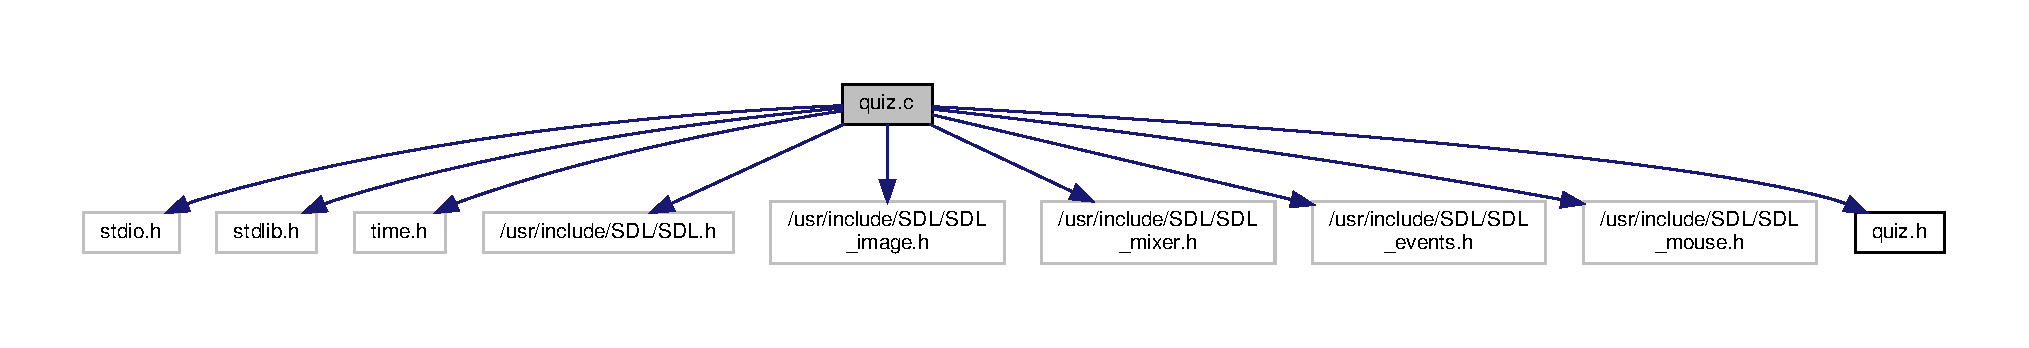
\includegraphics[width=350pt]{quiz_8c__incl}
\end{center}
\end{figure}
\subsection*{Functions}
\begin{DoxyCompactItemize}
\item 
int \hyperlink{quiz_8c_a8f387384696c4294f1521ad662b556db}{hover} (S\+D\+L\+\_\+\+Rect pos, int x, int y)
\item 
int \hyperlink{quiz_8c_a4fe6a4d28f2dc0d5df627aa0f7f86c65}{initialiser} (\hyperlink{structquiz}{quiz} $\ast$e, \hyperlink{structrest}{rest} $\ast$r)
\begin{DoxyCompactList}\small\item\em initialiser les donnees de l\textquotesingle{}enigme. \end{DoxyCompactList}\item 
void \hyperlink{quiz_8c_a161a7788abddb5e59234cd070e1bfa95}{afficher} (S\+D\+L\+\_\+\+Surface $\ast$screen, \hyperlink{structquiz}{quiz} e, \hyperlink{structrest}{rest} r, int var, int $\ast$vie, int $\ast$access)
\begin{DoxyCompactList}\small\item\em afficher et modifier les donnees de l\textquotesingle{}enigme. \end{DoxyCompactList}\end{DoxyCompactItemize}


\subsection{Detailed Description}
il y a ici tous les fonctions de l\textquotesingle{}enigme quiz. 



\subsection{Function Documentation}
\mbox{\Hypertarget{quiz_8c_a161a7788abddb5e59234cd070e1bfa95}\label{quiz_8c_a161a7788abddb5e59234cd070e1bfa95}} 
\index{quiz.\+c@{quiz.\+c}!afficher@{afficher}}
\index{afficher@{afficher}!quiz.\+c@{quiz.\+c}}
\subsubsection{\texorpdfstring{afficher()}{afficher()}}
{\footnotesize\ttfamily void afficher (\begin{DoxyParamCaption}\item[{S\+D\+L\+\_\+\+Surface $\ast$}]{screen,  }\item[{\hyperlink{structquiz}{quiz}}]{e,  }\item[{\hyperlink{structrest}{rest}}]{r,  }\item[{int}]{var,  }\item[{int $\ast$}]{vie,  }\item[{int $\ast$}]{access }\end{DoxyParamCaption})}



afficher et modifier les donnees de l\textquotesingle{}enigme. 


\begin{DoxyParams}{Parameters}
{\em S\+D\+L\+\_\+\+Surface} & $\ast$screen \+: affiche l\textquotesingle{}ecran. \\
\hline
{\em quiz} & e \+: utilise la structure obtenu di fichier binaire contien les questions et reponse. \\
\hline
{\em rest} & r\+: utilise la structure obtenu du fichier binaire contien interface et titre. \\
\hline
{\em S\+D\+L\+\_\+\+Event} & event \+: fait les actions generer pas le hardware. \\
\hline
{\em int} & var,$\ast$vie,$\ast$access \+: var est l aleatoire des enigmes vie et access depond si l\textquotesingle{}enigme est fini ou echouée. \\
\hline
\end{DoxyParams}
\begin{DoxyReturn}{Returns}
affichage de l\textquotesingle{}enigme. 
\end{DoxyReturn}
Here is the call graph for this function\+:\nopagebreak
\begin{figure}[H]
\begin{center}
\leavevmode
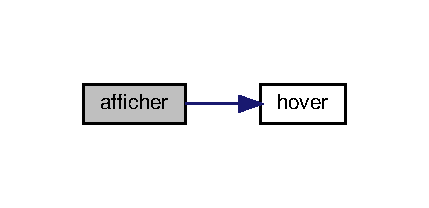
\includegraphics[width=206pt]{quiz_8c_a161a7788abddb5e59234cd070e1bfa95_cgraph}
\end{center}
\end{figure}
Here is the caller graph for this function\+:\nopagebreak
\begin{figure}[H]
\begin{center}
\leavevmode
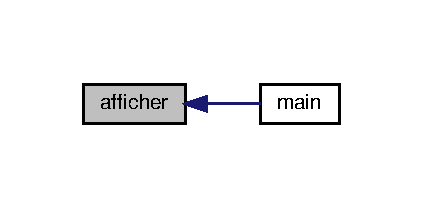
\includegraphics[width=203pt]{quiz_8c_a161a7788abddb5e59234cd070e1bfa95_icgraph}
\end{center}
\end{figure}
\mbox{\Hypertarget{quiz_8c_a8f387384696c4294f1521ad662b556db}\label{quiz_8c_a8f387384696c4294f1521ad662b556db}} 
\index{quiz.\+c@{quiz.\+c}!hover@{hover}}
\index{hover@{hover}!quiz.\+c@{quiz.\+c}}
\subsubsection{\texorpdfstring{hover()}{hover()}}
{\footnotesize\ttfamily int hover (\begin{DoxyParamCaption}\item[{S\+D\+L\+\_\+\+Rect}]{pos,  }\item[{int}]{x,  }\item[{int}]{y }\end{DoxyParamCaption})}

Here is the caller graph for this function\+:\nopagebreak
\begin{figure}[H]
\begin{center}
\leavevmode
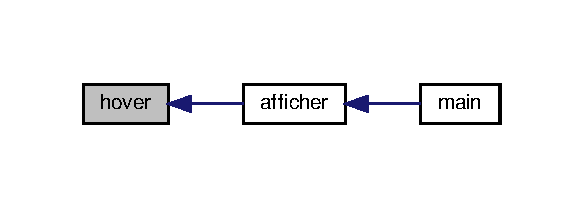
\includegraphics[width=280pt]{quiz_8c_a8f387384696c4294f1521ad662b556db_icgraph}
\end{center}
\end{figure}
\mbox{\Hypertarget{quiz_8c_a4fe6a4d28f2dc0d5df627aa0f7f86c65}\label{quiz_8c_a4fe6a4d28f2dc0d5df627aa0f7f86c65}} 
\index{quiz.\+c@{quiz.\+c}!initialiser@{initialiser}}
\index{initialiser@{initialiser}!quiz.\+c@{quiz.\+c}}
\subsubsection{\texorpdfstring{initialiser()}{initialiser()}}
{\footnotesize\ttfamily int initialiser (\begin{DoxyParamCaption}\item[{\hyperlink{structquiz}{quiz} $\ast$}]{e,  }\item[{\hyperlink{structrest}{rest} $\ast$}]{r }\end{DoxyParamCaption})}



initialiser les donnees de l\textquotesingle{}enigme. 


\begin{DoxyParams}{Parameters}
{\em quiz} & e \+: obtenir les fichiers binaires contien les questions et reponse. \\
\hline
{\em rest} & r\+: obtenir les fichiers binaires contien l\textquotesingle{}interface et titre. \\
\hline
\end{DoxyParams}
\begin{DoxyReturn}{Returns}
Initialisation de l\textquotesingle{}enigme 
\end{DoxyReturn}
Here is the caller graph for this function\+:\nopagebreak
\begin{figure}[H]
\begin{center}
\leavevmode
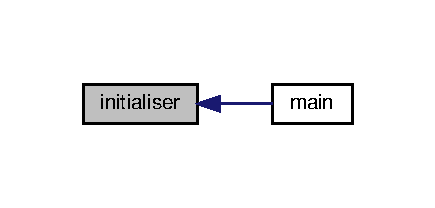
\includegraphics[width=209pt]{quiz_8c_a4fe6a4d28f2dc0d5df627aa0f7f86c65_icgraph}
\end{center}
\end{figure}

\hypertarget{quiz_8h}{}\section{quiz.\+h File Reference}
\label{quiz_8h}\index{quiz.\+h@{quiz.\+h}}


il y a ici les structures et la liaison des procedures de l\textquotesingle{}enigme.  


This graph shows which files directly or indirectly include this file\+:\nopagebreak
\begin{figure}[H]
\begin{center}
\leavevmode
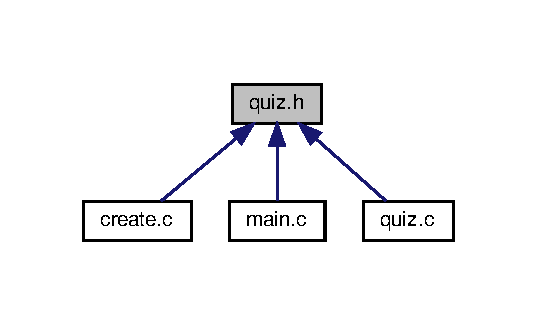
\includegraphics[width=258pt]{quiz_8h__dep__incl}
\end{center}
\end{figure}
\subsection*{Data Structures}
\begin{DoxyCompactItemize}
\item 
struct \hyperlink{structentity}{entity}
\item 
struct \hyperlink{structquiz}{quiz}
\item 
struct \hyperlink{structrest}{rest}
\end{DoxyCompactItemize}
\subsection*{Functions}
\begin{DoxyCompactItemize}
\item 
int \hyperlink{quiz_8h_a8f387384696c4294f1521ad662b556db}{hover} (S\+D\+L\+\_\+\+Rect pos, int x, int y)
\item 
int \hyperlink{quiz_8h_a4fe6a4d28f2dc0d5df627aa0f7f86c65}{initialiser} (\hyperlink{structquiz}{quiz} $\ast$e, \hyperlink{structrest}{rest} $\ast$r)
\begin{DoxyCompactList}\small\item\em initialiser les donnees de l\textquotesingle{}enigme. \end{DoxyCompactList}\item 
void \hyperlink{quiz_8h_a161a7788abddb5e59234cd070e1bfa95}{afficher} (S\+D\+L\+\_\+\+Surface $\ast$screen, \hyperlink{structquiz}{quiz} e, \hyperlink{structrest}{rest} r, int var, int $\ast$vie, int $\ast$access)
\begin{DoxyCompactList}\small\item\em afficher et modifier les donnees de l\textquotesingle{}enigme. \end{DoxyCompactList}\end{DoxyCompactItemize}


\subsection{Detailed Description}
il y a ici les structures et la liaison des procedures de l\textquotesingle{}enigme. 



\subsection{Function Documentation}
\mbox{\Hypertarget{quiz_8h_a161a7788abddb5e59234cd070e1bfa95}\label{quiz_8h_a161a7788abddb5e59234cd070e1bfa95}} 
\index{quiz.\+h@{quiz.\+h}!afficher@{afficher}}
\index{afficher@{afficher}!quiz.\+h@{quiz.\+h}}
\subsubsection{\texorpdfstring{afficher()}{afficher()}}
{\footnotesize\ttfamily void afficher (\begin{DoxyParamCaption}\item[{S\+D\+L\+\_\+\+Surface $\ast$}]{screen,  }\item[{\hyperlink{structquiz}{quiz}}]{e,  }\item[{\hyperlink{structrest}{rest}}]{r,  }\item[{int}]{var,  }\item[{int $\ast$}]{vie,  }\item[{int $\ast$}]{access }\end{DoxyParamCaption})}



afficher et modifier les donnees de l\textquotesingle{}enigme. 


\begin{DoxyParams}{Parameters}
{\em S\+D\+L\+\_\+\+Surface} & $\ast$screen \+: affiche l\textquotesingle{}ecran. \\
\hline
{\em quiz} & e \+: utilise la structure obtenu di fichier binaire contien les questions et reponse. \\
\hline
{\em rest} & r\+: utilise la structure obtenu du fichier binaire contien interface et titre. \\
\hline
{\em S\+D\+L\+\_\+\+Event} & event \+: fait les actions generer pas le hardware. \\
\hline
{\em int} & var,$\ast$vie,$\ast$access \+: var est l aleatoire des enigmes vie et access depond si l\textquotesingle{}enigme est fini ou echouée. \\
\hline
\end{DoxyParams}
\begin{DoxyReturn}{Returns}
affichage de l\textquotesingle{}enigme. 
\end{DoxyReturn}
Here is the call graph for this function\+:\nopagebreak
\begin{figure}[H]
\begin{center}
\leavevmode
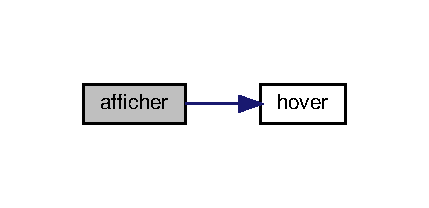
\includegraphics[width=206pt]{quiz_8h_a161a7788abddb5e59234cd070e1bfa95_cgraph}
\end{center}
\end{figure}
Here is the caller graph for this function\+:\nopagebreak
\begin{figure}[H]
\begin{center}
\leavevmode
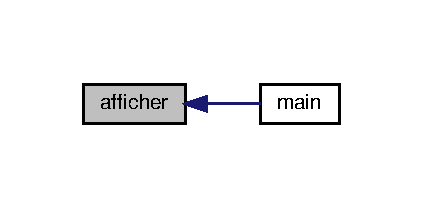
\includegraphics[width=203pt]{quiz_8h_a161a7788abddb5e59234cd070e1bfa95_icgraph}
\end{center}
\end{figure}
\mbox{\Hypertarget{quiz_8h_a8f387384696c4294f1521ad662b556db}\label{quiz_8h_a8f387384696c4294f1521ad662b556db}} 
\index{quiz.\+h@{quiz.\+h}!hover@{hover}}
\index{hover@{hover}!quiz.\+h@{quiz.\+h}}
\subsubsection{\texorpdfstring{hover()}{hover()}}
{\footnotesize\ttfamily int hover (\begin{DoxyParamCaption}\item[{S\+D\+L\+\_\+\+Rect}]{pos,  }\item[{int}]{x,  }\item[{int}]{y }\end{DoxyParamCaption})}

Here is the caller graph for this function\+:\nopagebreak
\begin{figure}[H]
\begin{center}
\leavevmode
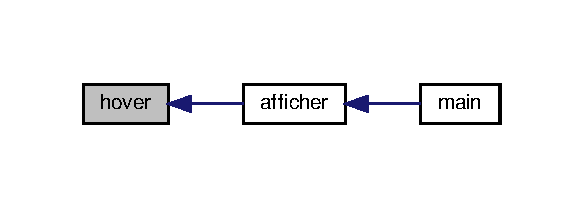
\includegraphics[width=280pt]{quiz_8h_a8f387384696c4294f1521ad662b556db_icgraph}
\end{center}
\end{figure}
\mbox{\Hypertarget{quiz_8h_a4fe6a4d28f2dc0d5df627aa0f7f86c65}\label{quiz_8h_a4fe6a4d28f2dc0d5df627aa0f7f86c65}} 
\index{quiz.\+h@{quiz.\+h}!initialiser@{initialiser}}
\index{initialiser@{initialiser}!quiz.\+h@{quiz.\+h}}
\subsubsection{\texorpdfstring{initialiser()}{initialiser()}}
{\footnotesize\ttfamily int initialiser (\begin{DoxyParamCaption}\item[{\hyperlink{structquiz}{quiz} $\ast$}]{e,  }\item[{\hyperlink{structrest}{rest} $\ast$}]{r }\end{DoxyParamCaption})}



initialiser les donnees de l\textquotesingle{}enigme. 


\begin{DoxyParams}{Parameters}
{\em quiz} & e \+: obtenir les fichiers binaires contien les questions et reponse. \\
\hline
{\em rest} & r\+: obtenir les fichiers binaires contien l\textquotesingle{}interface et titre. \\
\hline
\end{DoxyParams}
\begin{DoxyReturn}{Returns}
Initialisation de l\textquotesingle{}enigme 
\end{DoxyReturn}
Here is the caller graph for this function\+:\nopagebreak
\begin{figure}[H]
\begin{center}
\leavevmode
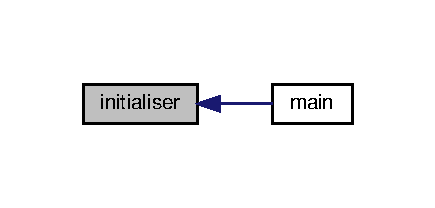
\includegraphics[width=209pt]{quiz_8h_a4fe6a4d28f2dc0d5df627aa0f7f86c65_icgraph}
\end{center}
\end{figure}

%--- End generated contents ---

% Index
\backmatter
\newpage
\phantomsection
\clearemptydoublepage
\addcontentsline{toc}{chapter}{Index}
\printindex

\end{document}
